\subsubsection{Example: Decomposing \texttt{mul}}\label{section:mul-example}

Consider the 32-bit number \texttt{0x71014802}. It is \emph{decomposed}
into fields of varying lengths depending on the \emph{format} of the
instruction.

For all numbers in the MIPS32 instruction set the leftmost six bits
always represent the opcode for the instruction. The opcode alone is
not always sufficient to identify the particular instruction,
\emph{but} it is always sufficient to identify the format of the
instruction.

The leftmost six bits of \texttt{0x71014802} is \texttt{0x1c}. It is
\emph{known} that this number corresponds to an instruction in the
R-format. The format specifies into which fields the remaining bits
decompose into. In Fig. \ref{fig:r-decomposed} each field's size in
bits is the small number below the field.

\begin{figure}[H]
  \centering
  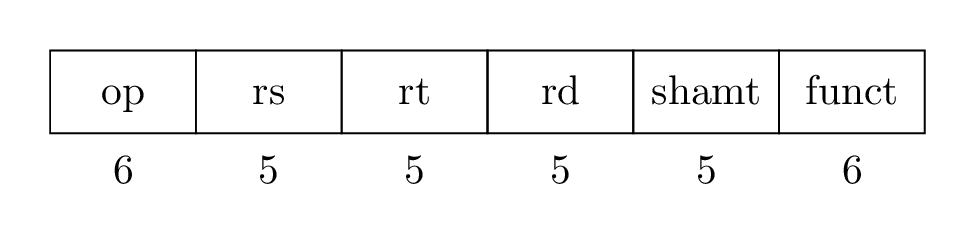
\includegraphics[width=0.9\textwidth]{figures/r-decomposed.png}
  \caption{The fields of an R-type instruction}
  \label{fig:r-decomposed}
\end{figure}

As alluded to previously, all instructions may not be discerned by
their opcode alone. This holds for all R-type instructions.

Decomposing \texttt{0x71014802} into the fields shown in
Fig. \ref{fig:r-decomposed} yields \texttt{rs=8}, \texttt{rt=1},
\texttt{rd=9}, \texttt{shamt=0}, and \texttt{funct=2}. The
\emph{decomposed representation} of this instruction in hexadecimal
form is thus \texttt{[0x1c 8 1 9 0 2]}.\footnote{The corresponding
\emph{decimal representation} is \texttt{[28 8 1 9 0 2]}}

To identify the particular instruction represented by
\texttt{0x71014802} the \texttt{funct} field must be
consulted. Pairing the opcode, \texttt{0x1c} and the value in the
\texttt{funct} field uniquely identifies the instruction a
\texttt{mul} instruction; see Fig. \ref{fig:mul-decomposed}

\begin{figure}[H]
  \centering
  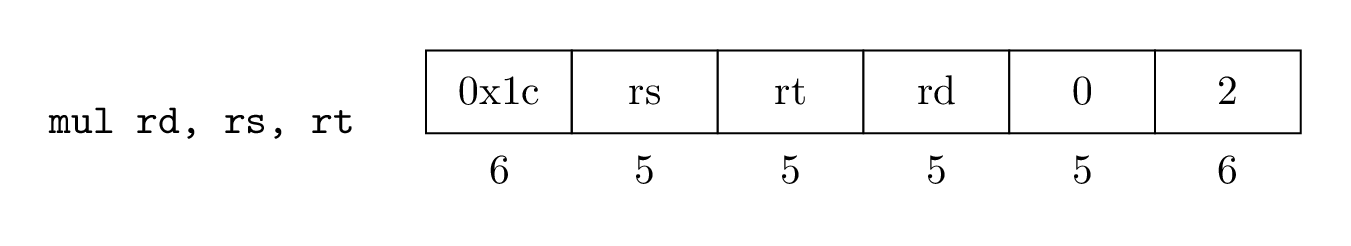
\includegraphics[width=0.9\textwidth]{figures/mul-decomposed.png}
  \caption{Decomposition and mnemonic representation of \texttt{mul}}
  \label{fig:mul-decomposed}
\end{figure}

From Fig. \ref{fig:r-decomposed} the registers \texttt{rs},
\texttt{rt} and \texttt{rd} were determined to have the addresses 8,
1, and 9, respectively. In MIPS registers are named, following the
convention shown in Table. \ref{table:mips-register-naming-convention}

\begin{table}[H]
\centering
\caption{MIPS register naming convention}
\begin{tabular}{ll}
\toprule
Nickname & Register Number \\
\midrule
\$zero      & 0            \\
\$at        & 1            \\
\$v0 - \$v1 & 2 - 3        \\
\$a0 - \$a3 & 4 - 7        \\
\$t0 - \$t7 & 8 - 15       \\
\$s0 - \$s7 & 16 - 23      \\
\$t8 - \$t9 & 24 - 25      \\
\$k0 - \$k1 & 26 - 27      \\
\$gp        & 28           \\
\$sp        & 29           \\
\$fp        & 30           \\
\$rd        & 31           \\
\bottomrule
\end{tabular}
\label{table:mips-register-naming-convention}
\end{table}

Replacing the numerical values of \texttt{rs}, \texttt{rt} and
\texttt{rd}, with their named counterparts yields the \emph{mnemonic
representation} of the instruction to be

\begin{center}
  \texttt{mul \$t1, \$t0, \$at}
\end{center}
